\section{Implementation}
\phantomsection
The initial step that was done, was the understanding of the purpose of the application. Different ideas had to be analyzed and decisions were made whether they should be included in the application or not. From the remaining set of ideas, some of them were labeled as a high priority and the others were decided to be considered as optional. Actually, this was done in order to set the developer on the right objectives. The high priority ideas, were considered essential for the application's main purpose. Given the time limit and the unforseen factors that could affect it, the most important tasks were to be developed first, leaving the other ones to be executed if there was time left. So, before beginning the implementation, QTK was conceptually divided into four main distinctive fragments:
\begin{enumerate}
  \item {User interface};
  \item {Quiz Managing};
  \item {Quiz generation};
  \item {Quiz processing}.
\end{enumerate}

These four elements of QTK will be amply described later in this chapter.

Ruby on Rails was the framework used in developing the web application. The default SQLite \cite{sqlite_doc} database, which was included in the generated Rails application, was considered to be sufficient for this thesis purpose and no other alternatives were searched. The following list of possibly to be used technologies was considered:
\begin{enumerate}
  \item Camellia;
  \item OpenCV;
  \item Tesseract;
  \item RMagick;
  \item ZBar;
  \item rqrcode;
  \item qrencoder;
  \item qrio;
  \item zxing;
  \item sidekiq;
  \item qrdecoder.
\end{enumerate}
Due to different reasons, most of these technologies were not used in the final version of the application to that is presented.

\subsection{User Interface}
The first step in creating the user interface, was to create the sketches of some of the web pages. The mockflow web app was used for this purpose. The figures \ref{fig3.1a} and \ref{fig3.1b} are the mockups based on which the real front-end was created.

\begin{figure}[!ht]
  \centering
  \subfloat[QTK's main page mockup\label{fig3.1a}]{%    
    \includegraphics[width=0.94\textwidth]{main_page_mockup}    
  }
 \hspace{0.09cm}
  \subfloat[QTK's quiz generation page mockup\label{fig3.1b}]{%
    \includegraphics[width=0.94\textwidth]{quiz_generate_mockup}
  }
  \caption{QTK's main page mockup (a), quiz generation page mockup (b).}
  \label{fig1.1}
\end{figure}


Bootstrap framework was used in developing the front-end of the application. Figures \ref{fig3.2a} and \ref{fig3.2b} illustrate the application of this framework in the QTK's user interface.


\begin{figure}[!ht]
  \centering
  \subfloat[QTK's main page\label{fig3.2a}]{%    
    \includegraphics[width=0.94\textwidth]{main_page_qtk}    
  }
 \hspace{0.09cm}
  \subfloat[QTK's generate quiz page\label{fig3.2b}]{%
    \includegraphics[width=0.94\textwidth]{generate_quiz_qtk}
  }
  \caption{QTK's main page (a), generate quiz page (b).}
  \label{fig1.1}
\end{figure}


The View layer, contain the templates, which are of ``Haml'' format(the default format is ``erb''). They constitute the interface which is displayed to the user. The contents can be text, images, tables, videos, hyperlinks and other elements which give the user the possibility to interact with the system. A haml formatted template which uses Bootstrap with CSS, HTML and JavaScript for styling is exemplified in listing \ref{new_question_haml}.

\lstinputlisting[language=Ruby, caption={Template \textit{new.html.haml} corresponding to action \textit{new} of QuestionsController}, label=new_question_haml]{../src/new.html.haml}

\subsection{Quiz managing}
Quiz managing covers a list of things:
\begin{itemize}
  \item Course creation, renaming and deletion;
  \item Quiz creation, renaming and deletion;
  \item Question creation, editing and deletion;
  \item Answer creation, editing and deletion;
  \item Question group creation and deletion.
\end{itemize}

These items, combined together, make the management system specific to QTK. They are implemented using the Rails framework and use all the layers proprietary to it. The model layer is used to create the classes representing the objects defined as course, quiz, question, answer and question group. A Model layer Question class example is given in listing \ref{question_class}.
The Controller, which serves as a bridge between the View and the Model layers contains the actions which react to the incoming requests. In listing \ref{students_class} is shown the StudentsController class. 

\lstinputlisting[language=Ruby, caption={Question class}, label=question_class]{../src/question.rb}

\lstinputlisting[language=Ruby, caption={StudentsController class}, label=students_class]{../src/students_controller.rb}

There is another type of classes which must be mentioned. The migration type classes inherit from the ActiveRecord::Migration class. The CreateAnswers class \ref{create_answers}, for example, is designed to create the table \textit{answers} in the database, with the specified fields. In this class, is indicated the foreign key of the table \textit{questions} which announces the relationship between these tables.


\lstinputlisting[language=Ruby, caption={CreateAnswers class}, label=create_answers]{../src/create_answers.rb}


\subsection{Quiz Generation}
Two gems(libraries) were additionally used to implement the ``quiz generation'' part of the application: Strokes and Prawn. Strokes is used to generate the QR codes and Prawn is used to generate the PDF files. The main idea was to give the user the possibility to generate the quizzes in different ways. So, options were provided for this purpose. Quizzes can be generated based on the chosen student groups, so the generated pdf would have copies created specifically for each student of those student groups. Or, the \textit{random} option can be choosed so the questions in every copy would be arranged in a random fashion.

When the user chooses to generate a quiz pdf, he selects the options he wants and sends the request to the server. Here, the \textit{GeneratedQuizzesController} class, which is responsible for catching this specific request, uses the \textit{create} method, defined in listing \ref{create_method}, to commence the generation process in the backend. 

\begin{lstlisting}[language=Ruby, caption={Create method of the GeneratedQuizzesController class}, label=create_method]
def create
  @user = current_user
  @generated_quiz = @user.generated_quizzes.new(generated_quiz_params)
  @generated_quiz.save
  GeneratedQuizzesHelper.gen_copies(@generated_quiz)
  # Generate pdf document
  pdf = QuizPdf.new(@generated_quiz)
  send_data pdf.render, filename: 'report.pdf', type: 'application/pdf', disposition: 'inline'
end
\end{lstlisting}

The \textit{GeneratedQuizzesHelper} module has a method named \textit{gen\_copies}, which is responsible for creating the necessary Copy class instances and persist them to the database, based on the options the user had chosen earlier. These options are contained in the variable passed as an arguement to this method. The necessity to create a separate method inside this module was because this process has its specific logic, which shouldn't be exposed in the controller action directly. By this, it is meant that some of the options were complementary, others were not. For example, the \textit{number of copies} option is interfering with the \textit{student group} option, because the second option's purpose is to create quiz copies based on the student's names, which in turn result in a determined number of final copies. Another option interference is the \textit{versions number} and the \textit{random} options. By selecting the number of versions to be generated for a quiz, it implies that each version will have the questions randomly sorted. So, once again, the other option becomes unnecessary to be selected.

The biggest role in the \textit{quiz generation} process has the \textit{QuizPdf} class. This class inherits from the \textit{Prawn::Document} class. It uses the Prawn's API to render all the required elements on the page. Here is a list of those elements: 
\begin{itemize}
  \item Questions;
  \item Answers;
  \item Squares next to the answers;
  \item The title
  \item Student name 
  \item Student group;
  \item QR code;
  \item Markers(circles) in each corner;
  \item Page number.
\end{itemize}

The \textit{set\_header} presented in listing \ref{set_header} of the \textit{QuizPdf} class is responsible for the QR code generation, title, student name, student group name and page number rendering and the stroking of the markers. 


\lstinputlisting[language=Ruby, caption={QuizPdf's \textit{set\_header} method}, label=set_header]{../src/set_header.rb}

The QR code is used to store some information in order to easily read it afterwards. In our case, the copy id of the \textit{Copy} class instance 
is encoded in the QR code. Also the current page number of the copy is stored in the QR code. This information will be critical in the later image processing part of the QTK's implementation. 

The markers, which are positioned at each corner of the generated quiz's page, are circles having a 10 pixel radius and a offset from the page's margins of 26 pixels on a 612x792 resolution pdf page. They are also going to be utilized in the image processing part, by using them as pivots when searching for the answer squares' coordinates.

The \textit{set\_questions} method is responsible for rendering the questions' and the answers' text. But, besides that, it draws the answers' squares, that are used by the students to select an answer when taking the quiz. Another thing related to the image processing is also being prepared at this point and that is the storing the ids of the questions and answers and the squares' left-top corner coordinates into a hash. At the end of the \textit{QuizPdf's} class execution, this hash is stored in the database in the copies table through the Copy class model. It is stored in the \textit{squares\_xy} field of that table.

After the \textit{QuizPdf} class instance is created and assigned to a variable, that instance is rendered into a pdf file in the web browser. Figure \ref{generated_quiz_page} shows an example of a generated quiz page. 

\begin{figure}[!ht]
\centering
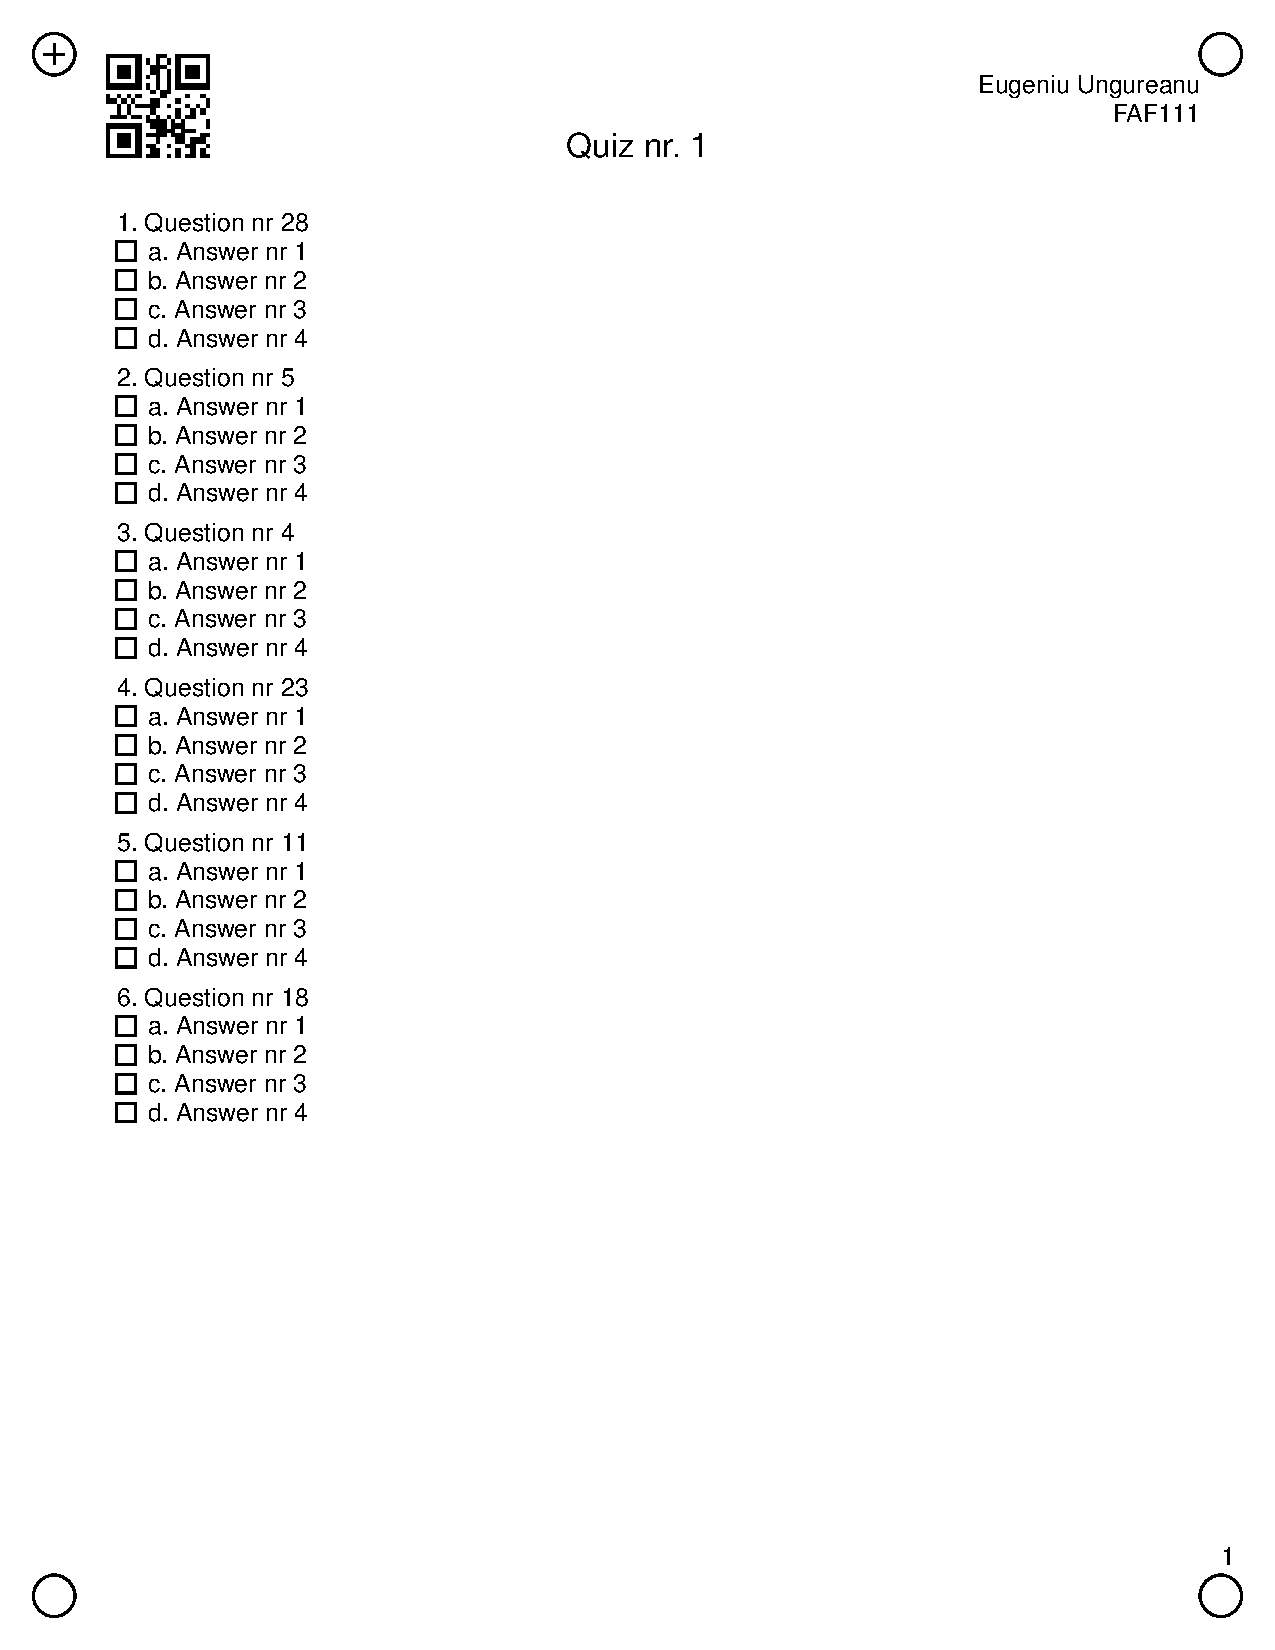
\includegraphics[width=\textwidth]{generated_quiz}
\caption{A generated quiz's page example}\label{generated_quiz_page}
\end{figure}


\subsection{Quiz Processing}

When the user uploads a set of files, which are the generated quizzes' scanned images, the system starts a background job for every one of them. These background jobs are the ones that do the image processing. 

The \textit{ScannedQuiz} model class found in listing \ref{scanned_quiz_class} is responsible for storing the metadata of one uploaded image per class instance and operates with the \textit{scanned\_quizzes} table in the database. But the first class to be accessed, when the user uploads something, is the UsersController class. It has the \textit{upload} action, which takes each image and creates a ScannedQuiz instance for it. At the model level, when these images are created and commited to the database, a callback is initiating a job. 

\lstinputlisting[language=Ruby, caption={ScannedQuiz class}, label=scanned_quiz_class]{../src/scanned_quiz.rb}

The \textit{ScansProcessingJob} is the class containing all the logic behind the processing of the images. The first method that should be mentioned, is \textit{read\_qr} in listing \ref{read_qr}. Reading the QR code's information is critical to the inception of the image processing. Whether it is read or not sets the processing to the next step or returns the specific error. The top-left corner of the image is cropped and passed to the \textit{ZBar::Image}(ZBar being the library used to decode QR codes) class for processing. The cropping is performed using the \textit{MiniMagick} library, which is a Ruby wrapper for \textit{ImageMagick} command line software. Also, in this method, is performed some image filtering and more specifically, the image is being thresholded by 60\%. The \textit{threshold} option provided by MiniMagick transforms a grayscale image, to a black and white one. 

\lstinputlisting[language=Ruby, caption={\textit{read\_qr} method}, label=read_qr]{../src/read_qr.rb}

The \textit{find\_marker} method shown in listing \ref{find_marker}, of the job processing class, is used to find the coordinates of the makers. It must receive three arguments in order to work and returns a hash containing the the coordinates for each pixel. The first argument is an object of type \textit{ChunkyPNG::Image}, which contains the rgb values of the entire image that was loaded. The other two arguments which must be given, are variables of \textit{Range} type, which represent the range of x axis and y axis that must be used to find the marker.  

\lstinputlisting[language=Ruby, caption={\textit{find\_marker} method}, label=find_marker]{../src/find_marker.rb}

Based on the found coodinates of the markers, the angle the page content is rotated can be calculated. First, the center coordinates of the bottom left and top left markers must be computed. These coordinates are passed to the \textit{rotation\_detection} method from listing \ref{rotation_detection}, which is responsible for getting the angle. The formula \ref{3.1} was used for computing the \textit{cosine} of $\alpha$ by using the vector's $v$ coordinates of the line formed by the centers of the two markers and vector $u$ which has the same $y$ value for all $x$.

\begin{equation}
\cos \alpha = \frac{\left\vert u_{1} \cdot v_{1} + u_{2} \cdot v_{2} \right\vert }{\sqrt{u_{1}^{2}+u_{2}^{2}} \cdot \sqrt{v_{1}^{2}+v_{2}^{2}}}  \label{3.1}
\end{equation}

where $u_{1}$ and $v_{1}$ represent the $x$ coordinates and $u_{2}$ and $v_{2}$ represent the $y$ coordinates of the vectors $v$ and $u$.

Since the angle is needed to be specified in radians, formula \ref{3.2} gets us the needed result.
\begin{equation}
radians = \arccos{\cos \alpha} \label{3.2}
\end{equation}

Actually, the angle in degrees is also calculated for testing purposes. Formula \ref{3.3} shows how the computation was made.

\begin{equation}
degrees = \frac{\arccos \cos \alpha \cdot 180}{\pi} \label{3.3}
\end{equation}

\lstinputlisting[language=Ruby, caption={\textit{rotation\_detection} method}, label=rotation_detection]{../src/rotation_detection.rb}


A part of the method \textit{answers\_processing} provided in listing \ref{answers_processing}, which uses data obtained from the previously mentioned methods, contains the logic behind identifying whether a certain square was marked or not in the scanned copy of the quiz. The \textit{copies} table's \textit{square\_xy} field's data is used to get the necessarry coordinates for each answer's square. Due to the possibility of the images' contents to be rotated to a certain degree, formulas \ref{3.4} and \ref{3.5}, which represent the rotation of a point in respect to (0, 0) point on the XY axis. where used to recalculate the current x and y coordinates of the square. 

\begin{equation}
x^{\prime} = x \cos \phi - y \sin \phi \label{3.4}
\end{equation}

\begin{equation}
y^{\prime} = y \cos \phi + x \sin \phi \label{3.5}
\end{equation}

where $\phi$ is the angle in radians calculated in formula \ref{3.2}

The pixels contained inside each square, are stored inside of an array. This is done using the \textit{ChunkyPNG's} possibility to access the images' pixels. Then the number of white and black pixels is calculated. The ratio black/white ratio number is used to determine whether the square was marked as anwer by the student or not. Squares which have the \textit{bw\_ratio} above 1 are considered as marked and are stored in another array that will be used in calculating the percentage of the correctly given answers.

\lstinputlisting[language=Ruby, caption={\textit{answers\_processing} method snippet}, label=answers_processing]{../src/answers_processing.rb}

In listing \ref{quiz_marking} is introduced the \textit{quiz\_marking} method. It's an implementation of the quizzes's grading based on its completion in percentage. It collects the correct answers ids from the database and compare them against the obtained ones. It offers one point for each correct answer. In the case when more than the necessary answers are given to a question, no points are given for any of those answers. The percentage obtained from the accumulated points is stored in the database.


\lstinputlisting[language=Ruby, caption={\textit{quiz\_marking} method}, label=quiz_marking]{../src/quiz_marking.rb}


The last method that is presented in listing \ref{perform} is the one which starts the image processing background job. It uses all of the methods mentioned in this subsection directly and indirectly.


\lstinputlisting[language=Ruby, caption={\textit{perform} method}, label=perform]{../src/perform.rb}

\clearpage